\documentclass[10pt]{article}
\usepackage{amsmath}
\usepackage{amssymb}
\usepackage{amsfonts}

\usepackage{enumerate}
\usepackage{array}
\usepackage{subfig}
\usepackage{graphicx}
\usepackage{float}

\usepackage{epstopdf}
\usepackage{multicol}
\usepackage{multirow}
\usepackage{authblk}

\usepackage{url}
\usepackage{cite}
\usepackage{booktabs}
\usepackage{titlesec}
\usepackage{titletoc}
\usepackage{epstopdf}
\usepackage[cm]{fullpage}

\usepackage{mathtools}
\usepackage{lscape}


\setlength{\parskip}{0ex plus0ex minus0ex}
%\setlength\parindent{10pt}
\setlength{\columnsep}{1cm}

\titleformat{\section}
  {\normalfont\sffamily\Large}
  {\thesection}{0.5em}{}
  
\titleformat{\subsection}
  {\normalfont\sffamily\large}
  {\thesubsection}{0.5em}{}

\titleformat{\subsubsection}
  {\normalfont\sffamily\normalsize}
  {\thesubsubsection}{0.5em}{}

\titlespacing*\section{0pt}{20pt plus 4pt minus 2pt}{5pt plus 2pt minus 2pt}
\titlespacing*\subsection{0pt}{16pt plus 4pt minus 2pt}{4pt plus 1pt minus 1pt}
\titlespacing*\subsubsection{0pt}{12pt plus 4pt minus 2pt}{2pt plus 0pt minus 0pt}

\renewcommand\thefigure{S\arabic{figure}}
\renewcommand\thetable{S\arabic{table}}
\renewcommand\thesection{S\arabic{section}}

\title{\vspace{-1.5cm}\sffamily Social fluidity mobilizes infectious disease in human and animal populations: supplementary information}
\date{}
\author[1]{Ewan Colman\footnote{ec975@georgetown.edu}}
\affil{\small{Department of Biology, Georgetown University, Washington, DC 20057, U.S.A}}
%\author[2]{Andreas Modlmeier}
%\author[2]{David Hughes}
%\affil{\small{Departments of Entomology and Biology, Penn State University, PA 16802, U.S.A}}
\author[1]{Shweta Bansal}
\renewcommand\Authands{ and }
\begin{document}
\maketitle
\vspace{-1cm}
{\sffamily\tableofcontents}
\hrulefill

\begin{multicols}{2}
\section{Measuring social fluidity}
Our analysis concerns a closed system containing a set $\mathcal{N}$ of $N$ individuals who can interact with each other in some way. The model has only one tunable parameter which we call ``social fluidity'' and can be interpreted as both the heterogeneity of relationship strengths, and the level of mixing in the population. From the description of the model we derive, analytically, the expected value of the the observed number of interaction partners of an individual, $d_{i}$, as a function of the number of times they been observed in an interaction, $s_{i}$. By using maximum likelihood methods we are able to measure and compare social fluidity quantity across a wide range of data.
 
\subsection{Mathematical model of social behavior}
\label{social_mixing}
We start by considering one focal individual $i$ and its relationship to another individual $j$. Suppose that $i$ is observed interacting with one other individual. We use  $x_{j|i}$, for all $j\in \mathcal{N}\setminus\{i\}$, to denote the probability that the interaction will be with $j$.
 
If at least one interaction has been observed between $i$ and $j$ then we say that an edge exists between them. The probability that this is the case after $i$ has been observed $s_{i}$ times is
\begin{equation}
\label{i_to_j_sup}
P(i \rightarrow j|s_{i})=1-(1-x_{j|i})^{s_{i}}.
\end{equation}

We now introduce heterogeneity into the distribution of relationship strengths. We make no assumptions about the relationship between $i$ and $j$ other than that $x_{j|i}$ is drawn from some distribution $\rho(x)$. The probability that an edge exists between $i$ and any node in the network after $s$ interactions is
\begin{equation}
\label{i_to_any_sup}
\Psi(s)=1-\int\rho(x)(1-x)^{s}dx.
\end{equation}
Letting $d_{i}$ be the degree of $i$, the expectation is simply $\mathbb{E}(d_{i})=(N-1)\psi(s_{i})$. For a given distribution ($\rho$) of relationship strengths in a population we now have a formula that connects the number of interactions to the degree.

Our goal is to choose the distribution $\rho$ that produces an accurate recreation of the behavior seen in real social systems. We therefore choose the truncated power law,
\begin{equation}
\label{distribution_sup}
\rho(x)=\frac{\phi\epsilon^{\phi}}{1-\epsilon^{\phi}}x^{-(1+\phi)} \text{ for } \epsilon<x<1.
\end{equation}
The reason for choosing a power law is that it allows the heterogeneity of the relationship strengths to be controlled by a single parameter $\phi$ making it adaptable to a wide variety of social systems. The distribution is truncated at $\epsilon$ so as not to include an asymptote at $x=0$. It is truncated $1$ to ensure that all values of $x_{j|i}$, which are probabilities, are less than $1$.

\subsection{Choosing $\epsilon$}
\label{epsilon}
The value of $\epsilon$ is determined by the choice of $\phi$. To find $\epsilon$, consider that interactions are pairwise; when $i$ interacts, exactly one other individual is involved. Hence, the expectation of the sum of the $x_{j|i}$'s over all $j\in \mathcal{N}\setminus\{i\}$ is equal to $1$. Another way to express this is
\begin{equation}
\label{sum_of_x}
(N-1) \langle x \rangle = 1
\end{equation}
where $\langle x \rangle$ denotes the mean of the distribution $\rho(x)$, and is
\begin{equation}
\label{x_mean}
\langle x \rangle=\frac{\phi\epsilon^{\phi}(1-\epsilon^{1-\phi})}{(1-\phi)(1-\epsilon^{\phi})}.
\end{equation}
Combining Eq.\eqref{sum_of_x} and Eq.\eqref{x_mean} we find that the only possible choice of $\epsilon$ is the solution of
\begin{equation}
(A+1)\epsilon^{\phi}-\epsilon-A=0
\end{equation}
where $A=(1-\phi)/(N-1)\phi$. 

\subsection{Degree distribution}
\label{degree_distribution}
Substituting Eq.\eqref{distribution_sup} into Eq.\eqref{i_to_any_sup} we have, for an individual that has had $s$ interactions, that
\begin{equation}
\Psi(s)=1-\frac{\phi\epsilon^{\phi}}{1-\epsilon^{\phi}}\int_{\epsilon}^{1} x^{-(1+\phi)}(1-x)^{s}dx.
\end{equation}
This simplifies to
\begin{equation}
\label{hyper_solution_sup}
\Psi(s)=1-\frac{\phi\epsilon^{\phi}(1-\epsilon)^{s+1}}{(1-\epsilon^{\phi})(s+1)}{}_{2}F_{1}(s+1, 1+\phi, s+2, 1-\epsilon)
\end{equation}
The notation ${}_{2}F_{1}$ refers to the Gauss hypergeometric function \cite{absteg}. Recall that $\Psi(s_{i})$ is the probability that an edge exists from $i$ to $j$, for any $j\in \mathcal{N}\setminus\{i\}$, after $i$ has been involved in $s_{i}$ interactions. The existence of any edge is therefore determined by a Bernoulli trial independent of the existence of any other. After $s$ interactions the degree of any node should therefore follow a binomial distribution $d(s)\sim B(N-1,\Psi(s))$, however, this gives non-zero probabilities for cases where $d>s$. This only occurs for $0<s<N$ so we replace the formula in this region with a binomial distribution with the same mean, $(N-1)\Psi(s)$, but bounded by $s$. Thus 
\begin{equation}
\label{binoms}
d_{i}(s) \sim
   \begin{dcases}
    B\left(s,\frac{(N-1)\Psi(s)}{s}\right) & \text{ if }0<s<N\\
    B\left(N-1,\Psi(s))\right) & \text{ if } s \geq N
  \end{dcases}
\end{equation}
\subsection{Estimating $\phi$ in empirical data}
\label{fitting}
The model we have described is based on the assumption that the system is closed; over some sampling period the $N$ individuals only interact with others from the same population. For each node $i$ we need to know know the number of time they interacted, $s_{i}$, and the number of others they interacted with, $d_{i}$. We write this as two vectors $\textbf{d}=\{d_{1},d_{2},...,d_{N}\}$ and $\textbf{s}=\{s_{1},s_{2},...,s_{N}\}$.

The family of distributions in Eq.\eqref{binoms} allow us to calculate $P(d|s)$, the probability that an individual will have degree $d$ given that they have interacted $s$ times, for any value of the global parameter $\phi$. The log-likelihood function is
\begin{equation}
\log \mathcal{L}(\phi|\textbf{d},\textbf{t})=\sum_{i=1}^{N}\log[P(d_{i}|s_{i})].
\end{equation}
We then compute the maximum likely estimate of $\phi$, $\phi=\text{argmax}_{\phi}\log \mathcal{L}(\phi|\textbf{d},\textbf{s})$. Standard error $SE_{\phi}$ is calculated at $95\%$ confidence intervals using $SE_{\phi}=1.96/\sqrt{-N(\log \mathcal{L})''}$ where the derivatives of $\log \mathcal{L}$ are computed numerically. The standard error is a measure of confidence that our chosen $\phi$ is in fact the best choice. It does not tell us how well the model fits the data in the first place. To quantify this we introduce a measure of model fidelity.

To measure model fidelity we compare the likelihood of the proposed model it to a null model that represents the most random, i.e. uniformly distributed, possible degree distribution for each given $t$. The null model equivalent of Eq.\eqref{binoms} is
\begin{equation}
\label{uniforms}
d(s) \sim 
   \begin{dcases}
    U(0,s) & \text{ if }0<s<N\\
    U(0,N-1) & \text{ if } s \geq N.
  \end{dcases}
\end{equation}
Model fidelity, $f_{\phi}$, quantifies the amount to which the proposed model fits the data when compared to an equivalent null model. We define it as
\begin{equation}
\label{fidelity}
f_{\phi}=(1/N)[\log \mathcal{L}(\phi|\textbf{d},\textbf{s})-\log \mathcal{L}(\text{null}|\textbf{d},\textbf{s})].
\end{equation}
Because we are using observed values of $s_{i}$ this approach controls for fact activity levels may vary between data sets.

Finally, to find a benchmark to compare the model fidelity we measured $f_{\phi}$ for several synthetically generated data sets. These data were generated by first selecting $100$ values of $s$ between $1$ and $100$ uniformly at random, then, for each one we select a value of $d$ either from the model distribution given by Eq.\eqref{binoms} or from the noise distribution given by Eq.\eqref{uniforms} ($N=100$ and $phi=0.6$). When less than $8\%$ of the synthetic values of $d$ come from the noise distribution, $f_{\phi}$ is positive. We conclude that positive values of $f_{\phi}$ found in any data-set implies that the model is a good fit to the data. 

%\begin{figure*}[t]
%\centering
%\subfloat[Caption text]{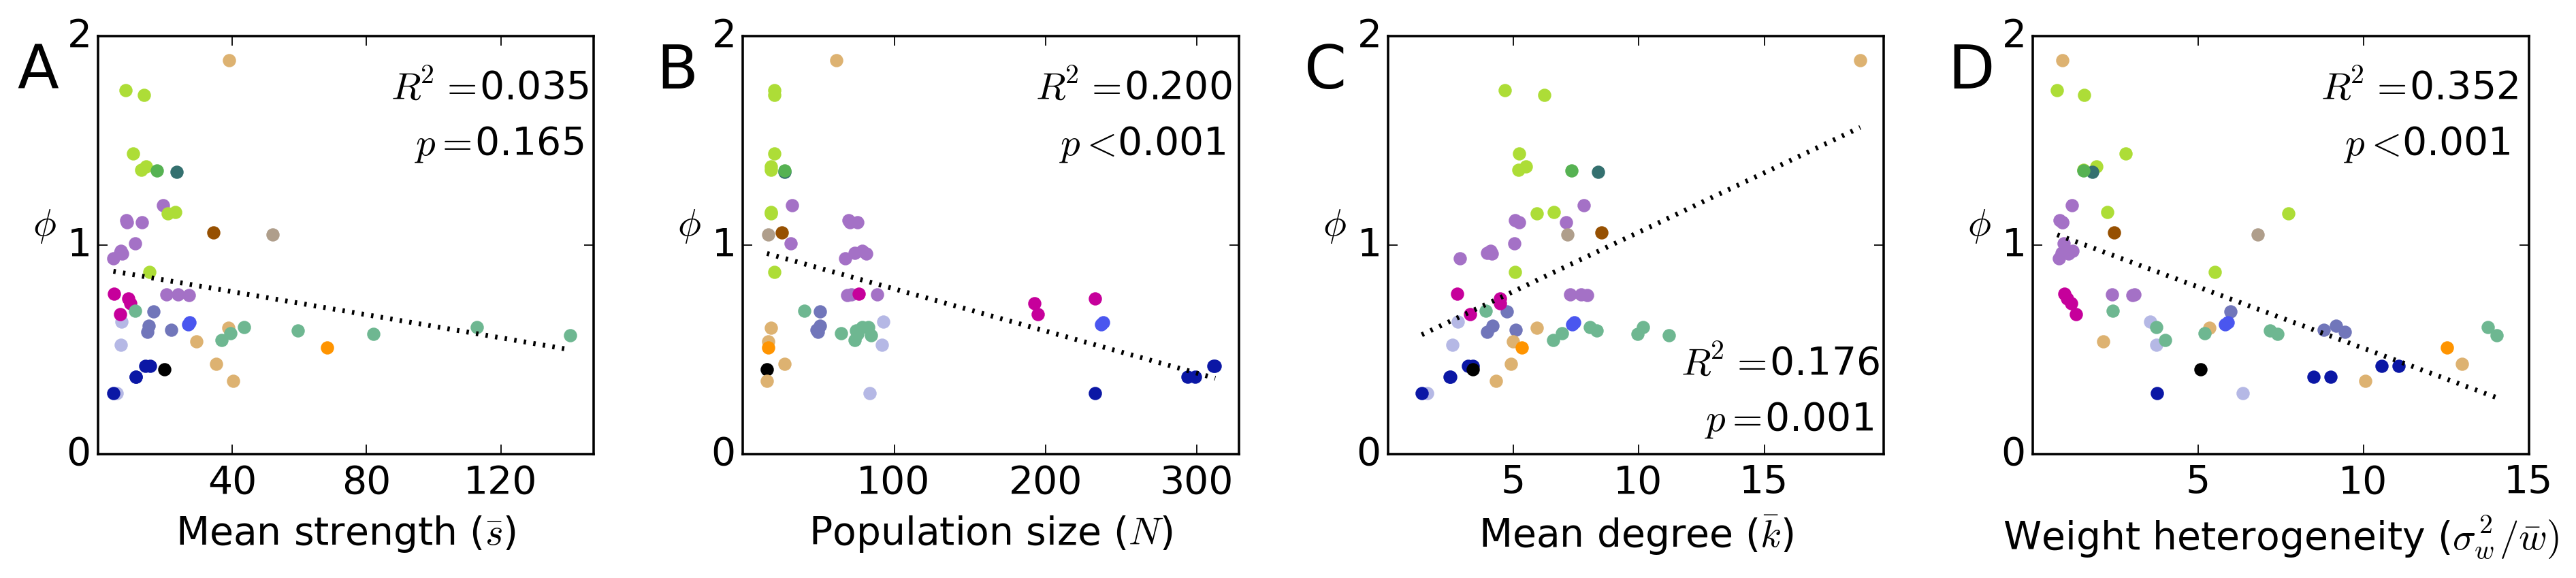
\includegraphics[height=7cm]{Figures/network_metrics.png}}\qquad
%\subfloat[Caption text]{\includegraphics[height=7cm]{Figures/Sociality_types.png}}
%\end{figure*}

\begin{figure*}[t]
	\centering
	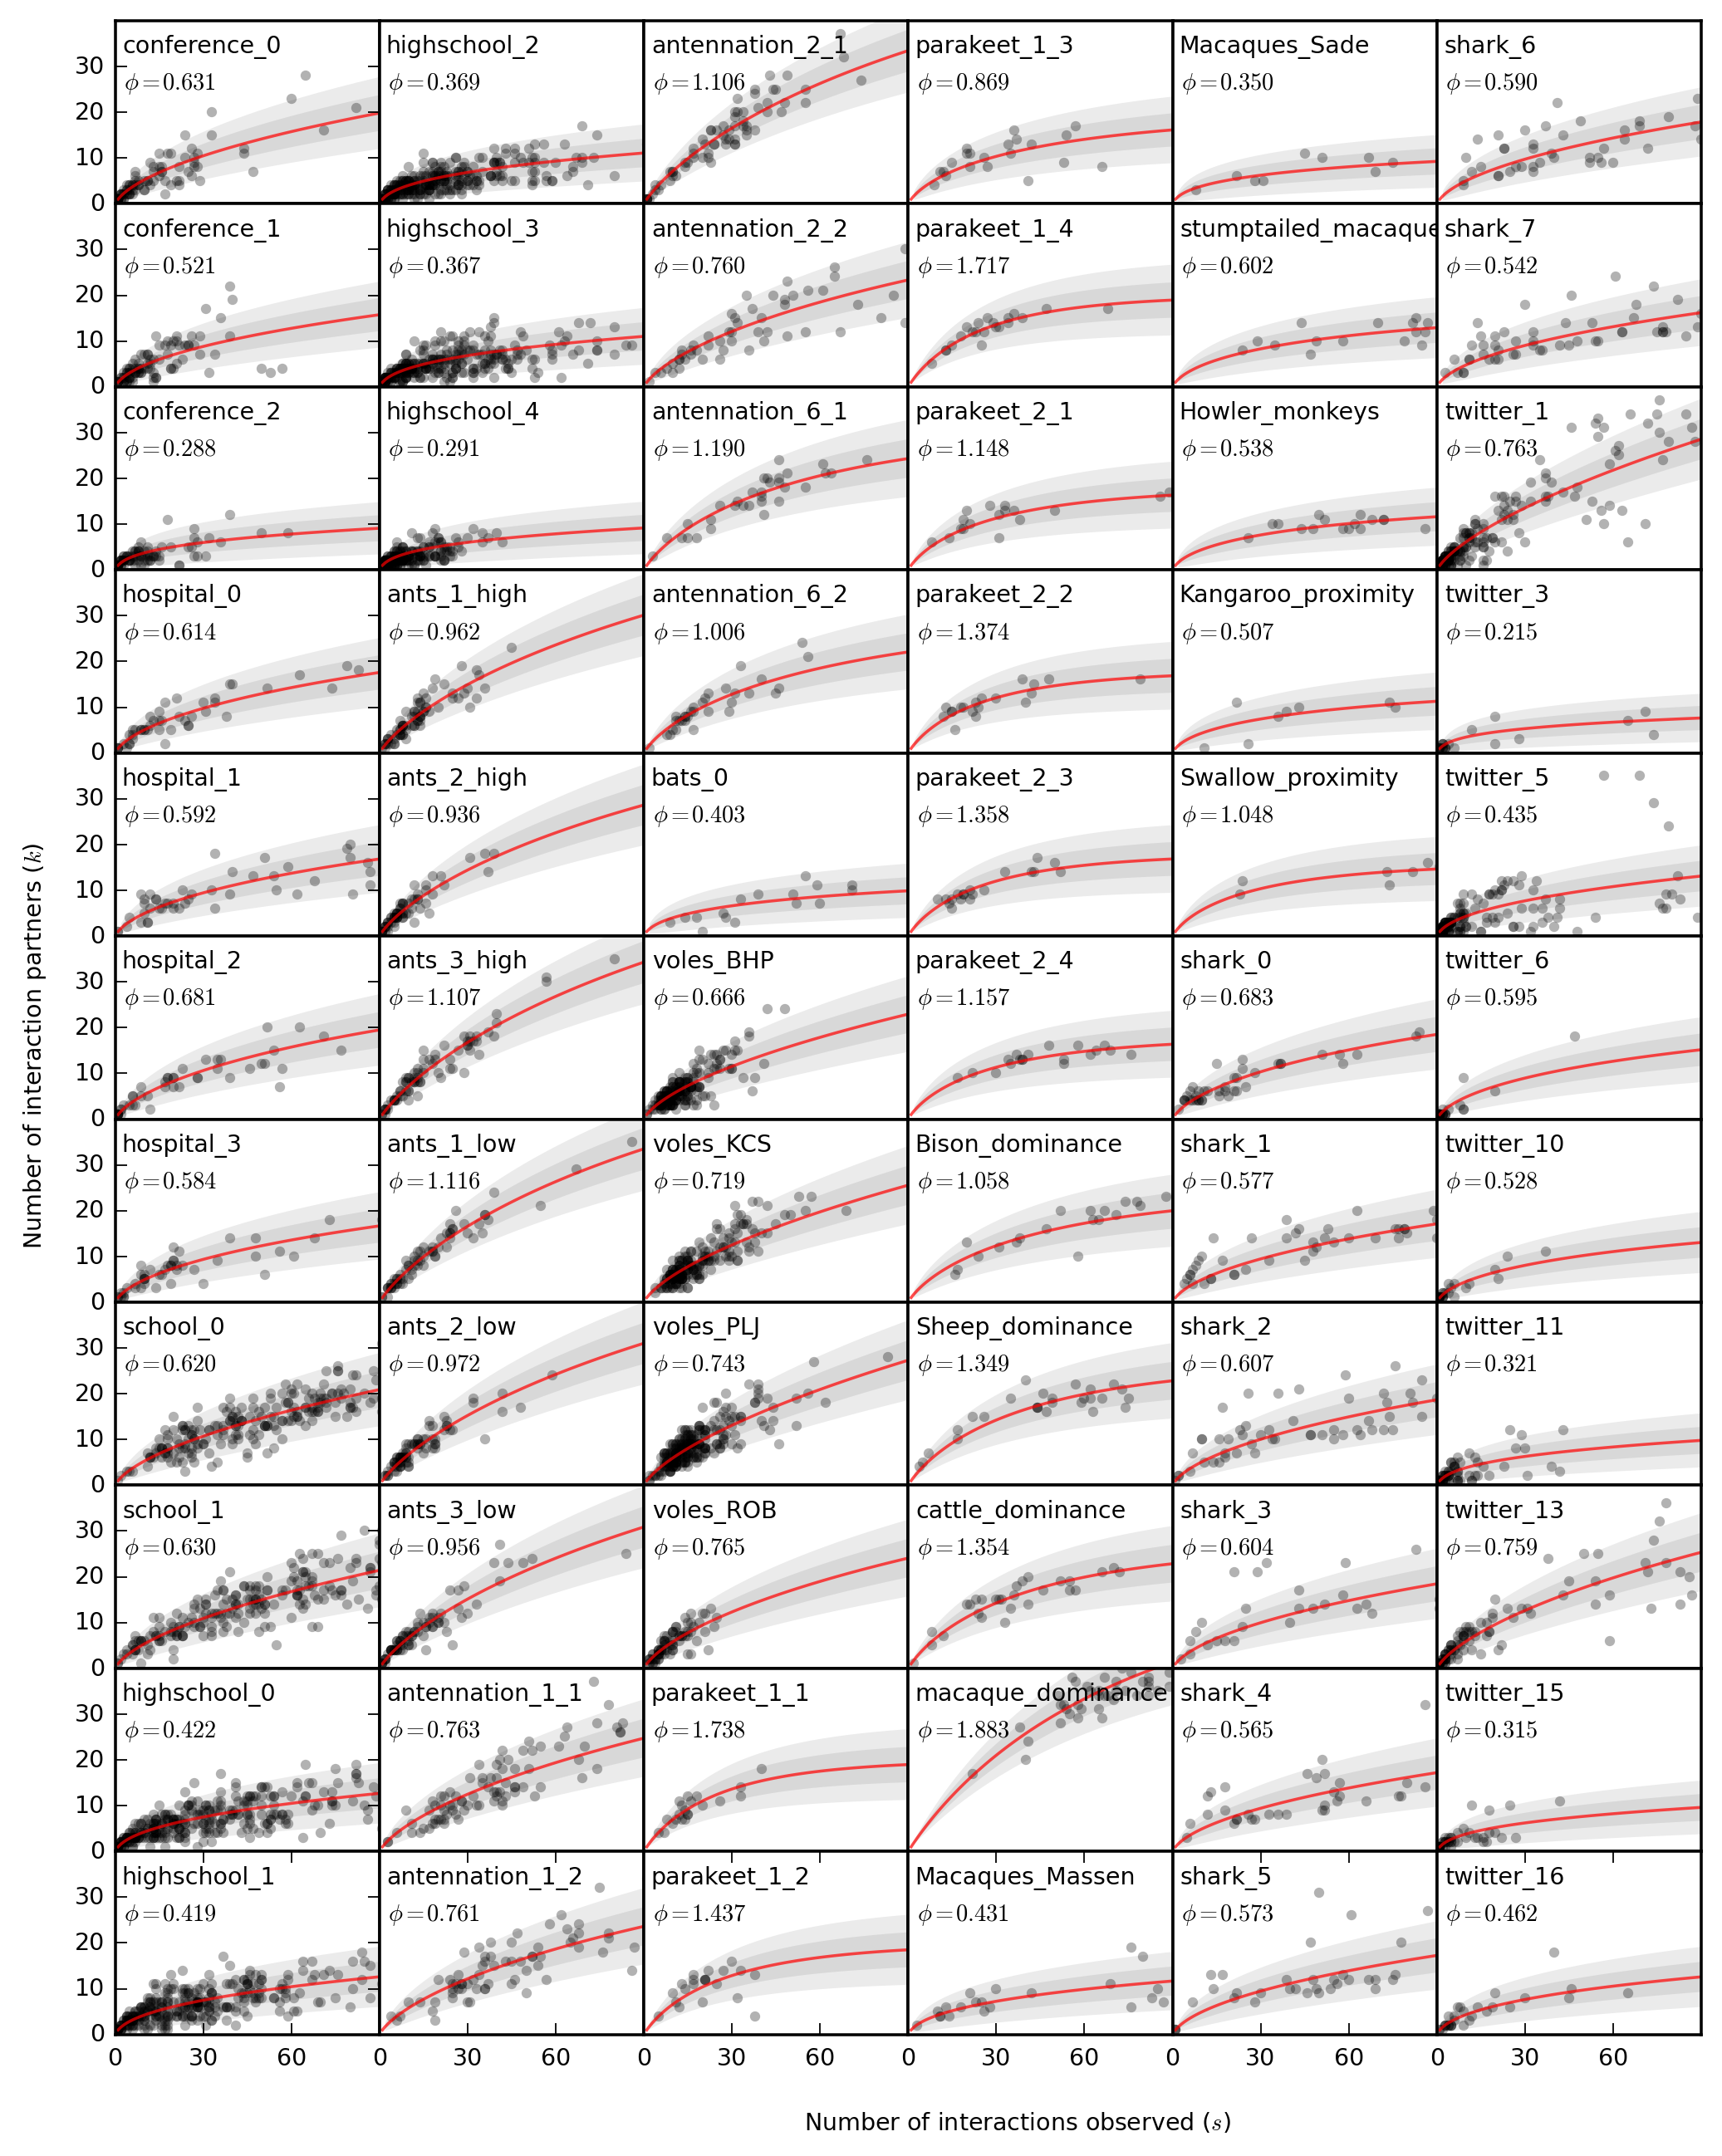
\includegraphics[width=\textwidth]{Figures/Degree_vs_int.png}
   	\caption{Every data-set used in our analysis as detailed in Section \ref{data}. Each point represents one individual in the system. In each case, the mixing parameter $\phi$ has been tuned to maximize the likelihood of the model using the process described in Section \ref{fitting}. The optimal $\phi$ is given and the curve shows the mean degree of an individual as a function of the number of interactions. The shaded area and the lighter shaded area represent intervals that are one and two standard deviations from the mean respectively. Data points for which the number of interactions is more than $90$ are excluded from the figure but not from the inference of $\phi$. [Reference the formulas that are in the text].}
\label{Degree_vs_int}
\end{figure*}

%%%%%%%%%%%%%%%%%%%%%%%%%%%%%%%%%%%%%%%%%%%%%%%%%%%%%%%%%%%%%%%%%%%%%%%%%%%%%%%%%%
\begin{table*}[t] 
\centering
\caption{Summary of parameters and variables}
\label{parameters}
\begin{tabular}{|c||c|}
\toprule
Social behavior & Disease transmission\\
\midrule
\begin{tabular}{r|p{7cm}}
 & \\
 $N$ & Number of nodes \\
$\sum s_{i}/2$ & The total number of interactions of all nodes \\
$\phi$ & The mixing parameter. The optimal value calculated from the process described in Section \ref{social_mixing} \\
$\epsilon$ & The lower cut-off for the relationship strength distribution, Eq.\eqref{distribution_sup} \\
$SE_{\phi}$ & The standard error of the estimate of $\phi$ \\
$f_{\phi}$ & Model fidelity. Given by Eq.\eqref{fidelity} \\
 & \\
\end{tabular}
&
\begin{tabular}{r|p{7cm}}
$\beta$ & The probability of transmission given that contact has occurred\\
 $\gamma$ & Recovery rate of the disease model. Chosen so that the mean number of infectious contacts is the same across all data-sets Eq.\eqref{gamma_sup}\\
$r_{i}$ & Mean individual reproduction number based on either Eq.\eqref{calibrated} or disease simulation.\\
$SE_{r}$ & Standard error of the reproduction number based on disease simulation\\
$|e|$ & Absolute error. Sum of the differences between $r_{i}$ predicted by Eq.\eqref{calibrated} and $r_{i}$ simulated \\
\end{tabular}\\
\bottomrule
\end{tabular}
\end{table*}
%%%%%%%%%%%%%%%%%%%%%%%%%%%%%%%%%%%%%%%%%%%%%%%%%%%%%%%%%%%%%%%%%%%%%%%%%%%%%%%%%%%%%%%%%%%%%%%%%%%%%%%%%%%%%%%%%%%%%%%%%

%%%%%%%%%%%%%%%%%%%%%%%%%%%%%%%%%%%%%%%%%%%%%%%%%%%%%%%%%%%%%%%%%%%%%%%%%%%%%%%%%%%%%%%%%%%%%%%%%%%%%%%%%%%%%%%%%%%%%%%%%
\section{Modelling the spread of disease}
The disease model is described as follows: We consider a fully susceptible population of $N$ individuals. At a randomly selected point in time, one individual, $i$, becomes infectious. They remain infectious for a duration of length $\tau$, where $\tau$ is a random variable drawn from an exponential distribution $P(\tau)=\gamma \exp(-\gamma \tau)$. This is equivalent to $i$ being able to recover at any point in time and $\gamma$ being the probability that recovery occurs at any point during an interval of length $1$. The times for which infected individual, $i$, engages in interaction follows a Poisson process with rate parameter $a_{i}$. Given that $i$ is engaged in an interaction, the probability that the interaction is with individual $j$ is $x_{j|i}$. Once contact is established, the probability that the disease will transmit is $\beta$.

\subsection{The number of secondary infections}
\label{disease_derivation}
We are interested in $r(a_{i})$, the expected number of other individuals infected by $i$, given that the rate of interaction of $i$ is $a_{i}$. 

The transmission probability, the probability that $i$ infects $j$ during an infectious period of length $\tau$, is equal to the probability that at $i$ makes infectious contact with $j$ at least once during that time. Since the rate of infectious contact between $i$ and $j$ follows a Poisson process with rate $a_{i}x_{j|i}\beta$, the transmission probability for an infectious period of length $\tau$ is derived from the Poisson distribution and is
\begin{equation}
T_{i\rightarrow j}(\tau,a_{i},x_{j|i})=1-\exp(a_{i}x_{j|i}\beta\tau).
\end{equation}
As in Section \ref{social_mixing} we make no assumptions about the relationship between $i$ and $j$ other than that $x_{j|i}$ is drawn from the distribution given by Eq.\eqref{distribution_sup}. The probability that transmission occurs from $i$ to any other node in the network is
\begin{equation}
\label{with_tau}
\begin{split}
T(\tau,a_{i})&=\int_{0}^{\infty}\rho(x)T_{i\rightarrow j}(\tau,a_{i},x)dx\\
&=1-\frac{\phi\epsilon^{\phi}}{1-\epsilon^{\phi}}\int_{\epsilon}^{1}x^{-(1+\phi)}\exp(a_{i}x_{j|i}\beta\tau)dx\\
&=1-\phi\sum_{k=0}^{\infty}\frac{(-a_{i}\beta\tau)^{k}}{(k-\phi)k!}\frac{\epsilon^{\phi}-\epsilon^{k}}{1-\epsilon^{\phi}}.
\end{split}
\end{equation}
The probability that $i$ was infectious for a period of duration $\tau$ is $\gamma\exp(-\gamma\tau)$. Integrating Eq.\eqref{with_tau} across all possible values of $\tau$ we get
\begin{equation}
\label{without_tau}
\begin{split}
T(a_{i})&=\int_{0}^{\infty}\gamma e^{-\gamma\tau}T_{i}(\tau,a_{i})d\tau\\
&=1-\phi\sum_{k=0}^{\infty}\frac{(-a_{i}\beta/\gamma)^{k}}{k-\phi}\frac{\epsilon^{\phi}-\epsilon^{k}}{1-\epsilon^{\phi}}.
\end{split}
\end{equation}
The quantity $T$ is the probability that $i$ will infect $j$ for any $j\in\mathcal{N}\setminus\{i\}$. To get the expected number of secondary infections that come from $i$ we simply have to multiply by the number of susceptibles. We therefore have that 
\begin{equation}
\label{r_i_1}
r(a_{i})=(N-1)T(a_{i}).
\end{equation}
It is not possible to express $T_{i}(a_{i})$ in terms of $N$ so we instead express it in terms of $\epsilon$. By substituting $N-1=1/\langle x \rangle$ and Eq.\eqref{x_mean} into Eq.\eqref{r_i_1} we get
\begin{equation}
\label{r_i}
\begin{split}
r(a_{i})&=\frac{T_{i}(a_{i})}{\langle x \rangle}\\
&=\frac{1-\phi}{\phi(\epsilon^{\phi}-\epsilon)}\left[1-\epsilon^{\phi}-\phi\sum_{k=0}^{k=\infty}\frac{(-a_{i}\beta/\gamma)^{k}}{k-\phi}(\epsilon^{\phi}-\epsilon^{k})\right]
\end{split}
\end{equation}
which can also be expressed using hypergeometric functions
\begin{equation}
\label{with_N}
\begin{split}
r(a_{i})=&\frac{1-\phi}{\phi(\epsilon^{\phi}-\epsilon)}\left[1-\epsilon^{\phi}+\epsilon^{\phi}{}_{2}F_{1}(-\phi,1,1-\phi;-a_{i}\beta/\gamma)\right.\\
&\left.-{}_{2}F_{1}(-\phi,1,1-\phi;-\epsilon a_{i}\beta/\gamma)\right]
\end{split}
\end{equation}
\subsection{Calibration of time-scales}
The collection of data-sets we compare is diverse and social activity happens on different time-scales. Additionally, the type of diseases that affect one species is unlikely to affect another. Instead of choosing parameter values that relate to some specific disease, it is more informative to select parameter values for each system separately in a way that exposes the effects of population size and social fluidity. To achieve this the two temporal variables, $\gamma$ and the mean activity rate, $\langle a_{i}\rangle$, are calibrated to each other in such a way that $R_{0}$ would always be the same value if, hypothetically, the effects of social fluidity and population size were not present.

We define $R^{*}$ to be the value of $R_{0}$ in a large population with homogenous mixing. In this case, the infectious individual, $i$, will never repeat an interaction with an individual whom they previously infected. In other words, every interaction during the infectious period will, with probability $\beta$, cause a new infection, and so $R^{*}$ can be found by multiplying the mean infectious period by $\beta$ and the mean rate interactions,
\begin{equation}
\label{R_star}
R^{*}=\frac{\beta\langle a_{i}\rangle}{\gamma}.
\end{equation}
By estimating the rate parameter $a_{i}$ from the number of observed interactions $s_{i}$ as $a_{i}=\frac{s_{i}}{\Delta_t}$ where $\Delta_{t}$ is the duration of the time-frame of the data, Eq.\eqref{R_star} becomes
\begin{equation}
\label{gamma}
\gamma=\frac{\beta\langle s\rangle}{\Delta_{t} R^{*}},
\end{equation}
where $\langle s\rangle$ is the mean of $s_{i}$ over all individuals. Additionally, by substituting this value of gamma into Eq.\eqref{with_N} we get
\begin{equation}
\label{calibrated}
\begin{split}
r(s)=&\frac{1-\phi}{\phi(\epsilon^{\phi}-\epsilon)}\left[1-\epsilon^{\phi}+\epsilon^{\phi}{}_{2}F_{1}(-\phi,1,1-\phi;-R^{*}s/\langle s \rangle)\right.\\
&\left.-{}_{2}F_{1}(-\phi,1,1-\phi;-\epsilon R^{*}s/\langle s \rangle)\right].
\end{split}
\end{equation}
Note that no temporal information appears in this equation. In all the analysis presented we have arbitrarily chosen $R^{*}=2$. 

\subsection{Limit of $R_{0}$ as $N\rightarrow \infty$}
Noting that the taking the limit in Eq.\eqref{r_i} as $\epsilon\rightarrow 0$ is equivalent to  $N\rightarrow \infty$ we can also say
\begin{equation} 
\label{big_N}
\lim_{N\rightarrow\infty}r_{i}(a_{i}) =\frac{1-\phi}{\phi}[-1+{}_{2}F_{1}(-\phi,1,1-\phi;-a_{i}\beta/\gamma) 
\end{equation}
if $\phi<1$ and 
\begin{equation}
\label{big_N2}
\lim_{N\rightarrow\infty}r_{i}(a_{i}) =a_{i}\beta/\gamma 
\end{equation}
if $\phi>1$ (at $\phi=1$, $\rho(x)$ is not defined). Arriving at this solution requires the use of L'Hopital's Rule.

\subsection{Simulating the spread of disease}
\label{simulation}
Because the fidelity of the social behavior model, i.e. the extent to which it agrees with the data, varies across the different social settings, we expect that the predictions made in Section \ref{disease_derivation} are only applicable to a some of our data-sets. To test how accurate the prediction of Eq.\eqref{with_N} is, we simulated the effects of transmission on the real contact data.

The collection of data-sets we are comparing is diverse, and social activity happens on dramatically different time-scales. To control for this variability the recovery rate $\gamma$ is adjusted. We choose $\gamma$ to be  
\begin{equation}
\label{gamma_sup}
\gamma=\frac{2\beta\sum t_{i}}{N \Delta_{t} s}
\end{equation}
where $\Delta_{t}$ is the duration of the time-frame of the data. Eq.\eqref{gamma_sup} is equivalent to choosing $\gamma$ such that, if the system is well-mixed, then an individual with the mean rate of activity is expected to directly infect $s$ others. In all the results presented we set $s=2$.

For every individual, $i$, the simulated reproduction number $r_{i}^{\text{sim}}$ is found by averaging the number of successful infections caused by $i$ over $10^{3}$ simulation trials. Each trial followed the following procedure:
\begin{enumerate}
\item A time $\tau$ is chosen randomly and uniformly between the beginning and end of the time-frame of the data
\item The length of infectious period $\Delta_{I}$ is generated from an exponential distribution with rate parameter $\gamma$
\item A list $L$ of interactions that involved $i$ between time $\tau$ and $\tau+\Delta_{I}$ is generated. If $\tau+\Delta_{I}$ is beyond the time-frame of the data then interactions from the beginning of the sampling time-frame are used in place of the missing data. 
\item Each interaction in the set $L$ is removed with probability $1-\beta$ and $r_{i}$ is the number of remaining individuals $j\in\mathcal{N}\setminus\{i\}$ that have interactions in $L$ 
\end{enumerate}
This gives a reproduction number for every individual in the system. In Table \ref{results_table} we provide the mean $\bar{r}$ and standard error $SE_{r}$ over the population. 

Finally, to measure the accuracy of Eq.\eqref{with_N} we calculate the mean absolute error $|e|$. We first calculate the rate of activity $a_{i}=t_{i}/\Delta_{t}$ which, along with the associated values of $N$, $phi$, and $\epsilon$, is used in Eq.\eqref{with_N} to compute $r_{i}$. The error is given by 
\begin{equation}
|e|=\frac{1}{N}\sum_{i\in\mathcal{N}}|r_{i}-r_{i}^{\text{sim}}|
\end{equation}

\section{Sources of empirical data}
\label{data}
\subsection{Human face-to-face interaction}
We use human contact data from the Sociopatterns project (sociopatterns.org). Participants wore radiofrequency identification sensors that detect face-to-face proximity of other participants within $1$-$1.5$ meters in $20$-second intervals. Each dataset lists the identities of the people in contact, as well as the $20$-second interval of detection. The timing and duration of contacts are known with a resolution of $20$-seconds. To exclude contacts detected while participants momentarily walked past one another, only contacts detected in at least two consecutive intervals are considered interactions.

The data we use comes from two studies: an academic conference which occurred over the course of $3$ days \cite{isella2011s}, a primary school for which there are $2$ days of data \cite{10.1371/journal.pone.0023176}, a high school which spanned $5$ days \cite{10.1371/journal.pone.0136497}, and a hospital which spanned $4$ full days \cite{10.1371/journal.pone.0073970}. In each case the data were divided into $24$ hour subsets beginning at midnight.

\subsection{Ant trophallaxis}
We collected data from three carpenter ant colonies (Camponotus Pennsylvanicus). In nature, carpenter ant foragers consume liquid food and, upon returning to the nest, regurgitate it into the mouths of their nest-mates, a process known as trophallaxis. Typically, foragers will only give food to a small number of other ants; to feed the entire colony it gets passed through a complex network of feeding interactions \cite{quevillon2015social}. Trophallaxis is also an important form of communication and a way that information about the state of the colony can be shared by all of its members \cite{greenwald2015ant,10.7554/eLife.20375}.

We placed colonies of approximately $80$ ants in a nest designed to replicate the conditions found in nature. The colony was first given a restrictive area of $65\times 42$mm to live (high density) the ants were given several days to adjust before $4$ hours of trophallaxis activity was recorded. The nest was then expanded by a factor of $4$ (low density) and after another adjustment period another $4$ hours were recorded. The process was repeated for $3$ unrelated colonies.

\subsection{Ant antennal Contact}
The antennae of ants contain highly sensitive olfactory cells. By touching the cuticle of another ant they are able to perceive information (primarily the status of the other ant) which is expressed through hydrocarbons secreted on their cuticle. We use data from \cite{10.1371/journal.pone.0020298} which was collected by constant human observation of video footage of ant colonies over a period of approximately 30 minutes. The experiment was performed on $3$ unrelated \emph{Temnothorax rugatulus} colonies, each of which was recorded in two sessions separated by a two week period.

%\subsection{Twitter mentions networks}
%Mentions on Twitter act as way to send messages directly to particular individuals. Although the message is broadcast to all the followers of the  account of the sender it will appear in the inbox of the receiver and is therefore likely to be noticed. Mentions often replied to \cite{10.1371/journal.pone.0022656}. We count an interaction as a reciprocated twitter mention, i.e. the motif A$\rightarrow$B, B$\rightarrow$A is an  interaction for A. We ignore all mentions that are not followed by reciprocation i.e. the motif A$\rightarrow$B, A$\rightarrow$B, B$\rightarrow$A, B$\rightarrow$A is counted as exactly $1$ interaction for A.

%In the study from which we take this data \cite{Charlton160162}, communities were first identified before their intensive data collection began. A range of community detection algorithms were used to decide which user accounts belong to the group and which do not, the goal being to find communities such that its members send messages within their community significant more than to user accounts outside the community. The $N$ individuals in the community form their own sub-population which acts somewhat like a closed system, a requisite for applying our analytical methods. 

%We use the last 24 hours of activity in each of the $17$ communities. We discard those for which the number of active users (during the $24$ hour period) is either less than $20$ or more than $250$.

%[Something about information transmission in social media]

\subsection{Bat food-sharing}
Vampire bats share food with each other through regurgitation. In order to initiate such an event a hungry bat will lick the mouth of another bat from whom they hope to receive food. The data we use is a record of mouth-licking observations originally collected to address questions of altruism and reciprocity in bat communities \cite{Carter20122573,dryad_tg7b1}.

A population of vampire bats (Desmodus rotundus) were kept captive in an enclosure. Out of the $25$ bats, $20$ were subjected to experimental treatment. In each case, the subject was removed from the enclosure and starved for $24$ hours. The observation period of $2$ hours began when the starved bat was let back into the enclosure and during this time the usual sources of food were not available. Thus, for the subject bat to feed, interaction with others was necessary. The starvation treatment and observations occurred on a different day for each bat. Some bats were tested more than once so to avoid biasing our results we select only the first day they were tested. 

\subsection{Vole territory sharing} 
Data were collected from a population of wild voles (Microtus agrestis) to assess the role of space in determining the structure of social networks \cite{Davis20141004}. [Sentence about vole behavior and what an interaction is].

In each of four field sites $100$ traps were placed in a square grid covering $0.3$ hectares. Bait was put into the traps and then three days later observers would check the traps for voles, those who were found were tagged so that they could be recognized should they be caught again. During each trapping session the traps were checked on several consecutive days. If a vole is observed in a trap at any point during a trapping session then we say that they interacted with any other vole that was observed in the same trap at any point during the same trapping session. The time of the interaction is the day that the trapping session began. 

We then discard any voles that had $10$ or less interactions and all interactions in which they participated. Since the voles have a very short lifespan and cyclic fluctuations in population size we use only a sub-sample of each data-set. We chose periods of $130$ days selected at times of high activity for each of the four experiment sites.

\subsection{Mouse territory sharing}
Mice \emph{Mastomys natalensis} \cite{borremans2016nonlinear} were kept in a large enclosed space that contained nine evenly spaced feeding stations. Four of nine feeding stations had sensors that recorded the moment when a mouse passed through its door. 

If two mice pass through within $30$ minutes of each other then we regard this as a territory sharing interaction comparable to the Vole data (in the source paper the authors used a 30 second threshold). The experiment was repeated with varying densities of mice, at low densities the very little interaction occurs so we use only the highest density treatments (enclosure C and enclosure D during the last 5 days).

\subsection{Association by group membership}
Since foraging groups and social groups can change from one day to the next, a commonly way to measure the strength of a pairwise relationship is to consider the number of times that the pair were observed in the same group. In most studies of this kind the data is processed in a way that attempts to correct for observation bias and group size heterogeneity, which makes it incompatible for our method of analysis. We were, however, able to use $3$ experiments from which the raw data is available. These are kangaroos \emph{Macropus giganteus} \cite{Grant1973449}, barn swallow \emph{Hirundo rustica erythrogaster}\cite{levin2016stress}, and howler monkeys \emph{Alouatta palliata} \cite{sailer1984proximity}. The data from each of these papers were collected through intermittent, rather than continuous, observation. We define an interaction as belonging to the same group during one round of observation.

\subsection{Grooming}
Grooming in monkeys, and other primates, is used to build and social bonds, avoid conflict, and maintain social structures including the dominance hierarchy. We used grooming data from two studies of macaques \emph{Macaca mulatta} \cite{massen2013stability,sade1972sociometrics} and one of stumptailed macaques \emph{Macaca arctoides} \cite{butovskaya1994structure}. Data were collected intermittently rather than through continuous observation. If one animal was grooming another during one round of observations then this would be recorded as a directed interaction. For our analysis we neglect the direction of the interaction (it is unclear whether the direction would have consequences relevant to the spread of disease).

\subsection{Aggression and dominance}
Aggression between animals can be in the form of a physical fight or a display of dominance that causes one individual to concede. From the literature we obtained aggression data from macaques \emph{Macaca fuscata fuscata} \cite{takahata1991diachronic}, female bighorn sheep \emph{Ovis canadensis} \cite{hass1991social}, bison \emph{Bison bison} \cite{lott1979dominance}, cattle \cite{SCHEIN195545}, and parakeets \emph{Myiopsitta monachus} \cite{hobson2015social}. The data from each of these papers were collected during intermittant observation periods. When an animal was determined to be the winner of a dominance encounter then this would be recorded as a directed interaction between the winner and the loser. For our analysis we neglect the direction of the interaction (it is unclear whether the direction would have consequences relevant to the spread of disease).
\end{multicols}

\begin{landscape}

\begin{table}[t]
\footnotesize
\caption{A description of each row header is given in Table \ref{parameters}}
\label{results_table}
\centering
\begin{tabular}{c|ccccccccccccc}
\toprule
Data set & System & Interaction & $N$ & $\sum s_{i}/2$ & $\sum d_{i}/2$ & $\sigma_{w}^{2}/\bar{w}$ & $\phi$ & $\epsilon \times 10^{3}$ & $f_{\phi}$ & $R_{0}$ (Pre.) & $\gamma \times 10^{4}$ & $R_{0}$ (Sim.) & Error \\ 
\midrule 
\verb|conference_0| & Conference & Face-to-face & $93$ & $663$ & $262$ & $5.946$ & $0.631$ & $0.356$ & $0.221$ & $1.254$ & $0.206$ & $1.178$ & $0.192$\\
\verb|conference_1| & Conference & Face-to-face & $92$ & $650$ & $239$ & $6.306$ & $0.521$ & $0.150$ & $0.016$ & $1.234$ & $0.204$ & $1.149$ & $0.258$\\
\verb|conference_2| & Conference & Face-to-face & $84$ & $477$ & $134$ & $9.790$ & $0.288$ & $0.005$ & $0.424$ & $1.054$ & $0.164$ & $0.879$ & $0.215$\\
\verb|hospital_0| & Hospital & Face-to-face & $51$ & $778$ & $213$ & $12.225$ & $0.614$ & $0.878$ & $0.769$ & $1.223$ & $0.441$ & $1.142$ & $0.130$\\
\verb|hospital_1| & Hospital & Face-to-face & $49$ & $1075$ & $250$ & $12.201$ & $0.592$ & $0.825$ & $0.845$ & $1.239$ & $0.635$ & $1.142$ & $0.165$\\
\verb|hospital_2| & Hospital & Face-to-face & $51$ & $855$ & $242$ & $8.849$ & $0.681$ & $1.244$ & $0.803$ & $1.279$ & $0.485$ & $1.253$ & $0.123$\\
\verb|hospital_3| & Hospital & Face-to-face & $50$ & $743$ & $198$ & $12.585$ & $0.584$ & $0.759$ & $0.713$ & $1.213$ & $0.430$ & $1.141$ & $0.136$\\
\verb|school_0| & Primary school & Face-to-face & $237$ & $6420$ & $1744$ & $9.267$ & $0.620$ & $0.070$ & $1.245$ & $1.378$ & $0.784$ & $1.299$ & $0.142$\\
\verb|school_1| & Primary school & Face-to-face & $238$ & $6514$ & $1769$ & $9.367$ & $0.630$ & $0.076$ & $1.148$ & $1.368$ & $0.792$ & $1.288$ & $0.146$\\
\verb|highschool_0| & High school & Face-to-face & $312$ & $4919$ & $1058$ & $15.620$ & $0.422$ & $0.003$ & $0.830$ & $1.175$ & $0.456$ & $0.990$ & $0.228$\\
\verb|highschool_1| & High school & Face-to-face & $311$ & $4419$ & $997$ & $14.894$ & $0.419$ & $0.002$ & $0.685$ & $1.167$ & $0.411$ & $0.982$ & $0.228$\\
\verb|highschool_2| & High school & Face-to-face & $299$ & $3415$ & $746$ & $13.011$ & $0.369$ & $0.001$ & $0.765$ & $1.129$ & $0.330$ & $0.953$ & $0.222$\\
\verb|highschool_3| & High school & Face-to-face & $294$ & $3331$ & $732$ & $13.483$ & $0.367$ & $0.001$ & $0.669$ & $1.130$ & $0.328$ & $0.954$ & $0.229$\\
\verb|highschool_4| & High school & Face-to-face & $233$ & $1084$ & $316$ & $7.154$ & $0.291$ & $0.000$ & $0.345$ & $1.073$ & $0.135$ & $0.833$ & $0.252$\\
\verb|ants_1_high| & Ant & Food sharing & $74$ & $496$ & $293$ & $2.401$ & $0.962$ & $2.030$ & $0.450$ & $1.556$ & $1.164$ & $1.506$ & $0.138$\\
\verb|ants_2_high| & Ant & Food sharing & $68$ & $318$ & $196$ & $2.282$ & $0.936$ & $2.105$ & $0.427$ & $1.506$ & $0.812$ & $1.325$ & $0.187$\\
\verb|ants_3_high| & Ant & Food sharing & $76$ & $674$ & $399$ & $2.351$ & $1.107$ & $2.752$ & $0.655$ & $1.615$ & $1.540$ & $1.599$ & $0.123$\\
\verb|ants_1_low| & Ant & Food sharing & $70$ & $606$ & $356$ & $2.277$ & $1.116$ & $3.075$ & $0.782$ & $1.606$ & $1.503$ & $1.611$ & $0.100$\\
\verb|ants_2_low| & Ant & Food sharing & $79$ & $547$ & $324$ & $2.731$ & $0.972$ & $1.926$ & $0.626$ & $1.561$ & $1.202$ & $1.494$ & $0.115$\\
\verb|ants_3_low| & Ant & Food sharing & $82$ & $610$ & $342$ & $2.695$ & $0.956$ & $1.763$ & $0.548$ & $1.525$ & $1.291$ & $1.492$ & $0.117$\\
\verb|Blonder_ants_1_1| & Ant & Antennal contact & $89$ & $1834$ & $649$ & $4.756$ & $0.763$ & $0.794$ & $0.806$ & $1.461$ & $35.825$ & $1.539$ & $0.157$\\
\verb|Blonder_ants_1_2| & Ant & Antennal contact & $72$ & $1721$ & $556$ & $5.516$ & $0.761$ & $1.065$ & $0.763$ & $1.450$ & $34.166$ & $1.538$ & $0.135$\\
\verb|Blonder_ants_2_1| & Ant & Antennal contact & $71$ & $943$ & $505$ & $2.391$ & $1.106$ & $2.970$ & $0.825$ & $1.631$ & $23.091$ & $1.700$ & $0.107$\\
\verb|Blonder_ants_2_2| & Ant & Antennal contact & $69$ & $1880$ & $549$ & $5.644$ & $0.760$ & $1.124$ & $0.810$ & $1.416$ & $37.926$ & $1.534$ & $0.174$\\
\verb|Blonder_ants_6_1| & Ant & Antennal contact & $33$ & $647$ & $258$ & $2.467$ & $1.190$ & $8.320$ & $1.105$ & $1.604$ & $25.555$ & $1.716$ & $0.117$\\
\verb|Blonder_ants_6_2| & Ant & Antennal contact & $32$ & $362$ & $162$ & $2.458$ & $1.006$ & $6.407$ & $0.751$ & $1.516$ & $16.115$ & $1.602$ & $0.122$\\
\verb|bats_0| & Bat & Food sharing & $16$ & $290$ & $54$ & $9.236$ & $0.427$ & $3.105$ & $0.640$ & $1.228$ & $6.380$ & $1.077$ & $0.344$\\
\verb|voles_BHP| & Vole & Territorial & $195$ & $1339$ & $640$ & $3.332$ & $0.666$ & $0.141$ & $0.368$ & $1.412$ & $132.051$ & $1.374$ & $0.166$\\
\verb|voles_KCS| & Vole & Territorial & $193$ & $1874$ & $865$ & $3.236$ & $0.719$ & $0.206$ & $0.632$ & $1.459$ & $186.728$ & $1.498$ & $0.148$\\
\verb|voles_PLJ| & Vole & Territorial & $233$ & $2126$ & $1048$ & $2.991$ & $0.743$ & $0.183$ & $0.448$ & $1.476$ & $175.470$ & $1.519$ & $0.145$\\
\verb|voles_ROB| & Vole & Territorial & $77$ & $381$ & $214$ & $2.613$ & $0.765$ & $0.982$ & $0.243$ & $1.454$ & $95.155$ & $1.291$ & $0.179$\\
\verb|mice_C_5| & Mouse & Territorial & $57$ & $665$ & $242$ & $4.075$ & $0.674$ & $1.008$ & $0.957$ & $1.354$ & $0.125$ & $1.219$ & $0.188$\\
\verb|mice_D_5| & Mouse & Territorial & $41$ & $404$ & $138$ & $4.587$ & $0.653$ & $1.550$ & $0.800$ & $1.251$ & $0.105$ & $1.336$ & $0.136$\\
\verb|parakeet_1_1| & Parakeet & Aggression & $21$ & $175$ & $98$ & $0.742$ & $1.738$ & $22.574$ & $0.738$ & $1.671$ & $nan$ & $nan$ & $nan$\\
\verb|parakeet_1_2| & Parakeet & Aggression & $21$ & $222$ & $110$ & $2.826$ & $1.437$ & $18.361$ & $0.061$ & $1.619$ & $nan$ & $nan$ & $nan$\\
\verb|parakeet_1_3| & Parakeet & Aggression & $21$ & $325$ & $107$ & $5.518$ & $0.869$ & $8.568$ & $0.268$ & $1.446$ & $nan$ & $nan$ & $nan$\\
\verb|parakeet_1_4| & Parakeet & Aggression & $21$ & $291$ & $131$ & $1.573$ & $1.717$ & $22.304$ & $1.151$ & $1.675$ & $nan$ & $nan$ & $nan$\\
\verb|parakeet_2_1| & Parakeet & Aggression & $19$ & $399$ & $113$ & $7.737$ & $1.148$ & $15.418$ & $0.878$ & $1.532$ & $nan$ & $nan$ & $nan$\\
\verb|parakeet_2_2| & Parakeet & Aggression & $19$ & $273$ & $105$ & $1.931$ & $1.374$ & $19.537$ & $0.957$ & $1.593$ & $nan$ & $nan$ & $nan$\\
\verb|parakeet_2_3| & Parakeet & Aggression & $19$ & $247$ & $99$ & $1.552$ & $1.358$ & $19.266$ & $1.032$ & $1.588$ & $nan$ & $nan$ & $nan$\\
\verb|parakeet_2_4| & Parakeet & Aggression & $19$ & $441$ & $126$ & $2.267$ & $1.157$ & $15.592$ & $1.204$ & $1.551$ & $nan$ & $nan$ & $nan$\\
\verb|Bison_dominance| & Bison & Aggression & $26$ & $897$ & $222$ & $2.467$ & $1.058$ & $9.130$ & $0.884$ & $1.546$ & $nan$ & $nan$ & $nan$\\
\verb|Sheep_dominance| & Sheep & Aggression & $28$ & $658$ & $235$ & $1.806$ & $1.349$ & $12.166$ & $0.940$ & $1.649$ & $nan$ & $nan$ & $nan$\\
\verb|cattle_dominance| & Cattle & Aggression & $28$ & $498$ & $205$ & $1.544$ & $1.354$ & $12.230$ & $0.946$ & $1.647$ & $nan$ & $nan$ & $nan$\\
\verb|macaque_dominance| & Monkey & Aggression & $62$ & $2435$ & $1167$ & $0.908$ & $1.883$ & $7.795$ & $1.442$ & $1.860$ & $nan$ & $nan$ & $nan$\\
\verb|Macaques_Massen| & Monkey & Grooming & $28$ & $2025$ & $228$ & $15.949$ & $0.523$ & $1.573$ & $1.913$ & $1.320$ & $nan$ & $nan$ & $nan$\\
\verb|Macaques_Sade| & Monkey & Grooming & $16$ & $647$ & $69$ & $10.074$ & $0.350$ & $1.917$ & $0.912$ & $1.208$ & $nan$ & $nan$ & $nan$\\
\verb|stumptailed_macaque| & Monkey & Grooming & $19$ & $742$ & $113$ & $5.351$ & $0.602$ & $4.776$ & $0.958$ & $1.344$ & $nan$ & $nan$ & $nan$\\
\verb|Howler_monkeys| & Monkey & Association & $17$ & $502$ & $85$ & $2.135$ & $0.538$ & $4.605$ & $1.009$ & $1.321$ & $nan$ & $nan$ & $nan$\\
\verb|Kangaroo_proximity| & Kangaroo & Association & $17$ & $1161$ & $91$ & $12.532$ & $0.507$ & $4.030$ & $1.247$ & $1.245$ & $nan$ & $nan$ & $nan$\\
\verb|Swallow_proximity| & Swallow & Association & $17$ & $886$ & $122$ & $6.808$ & $1.048$ & $15.619$ & $1.578$ & $1.505$ & $nan$ & $nan$ & $nan$\\
\bottomrule
\end{tabular}
\end{table}

\end{landscape}

\small
\bibliography{bibfile}
\bibliographystyle{ieeetr}
\normalsize

\end{document}
